% =====================================================================
% Cross-Lingual Memory in LLM Agents (course project paper, midsem)
% Template: course ACL template, LuaLaTeX variant (needed for Devanagari).
% COMPILE WITH LuaLaTeX  (Overleaf: Menu > Compiler > LuaLaTeX).
% =====================================================================
\documentclass[11pt]{article}

% "final" shows author names. Use "review" for an anonymous version.
\usepackage[final]{acl}
\usepackage{microtype}

% Hindi requires Unicode shaping. Select LuaLaTeX in Overleaf before compiling.
\usepackage{iftex}
\ifLuaTeX\else
  \PackageError{main.tex}{Compile this document with LuaLaTeX}{In Overleaf, select Menu > Compiler > LuaLaTeX, then recompile. pdfLaTeX cannot render the Hindi Unicode text in this paper.}
  \expandafter\endinput
\fi
\usepackage[english,bidi=default]{babel}
\babelfont{rm}{TeXGyreTermesX}
\babelprovide[import, onchar=ids fonts]{hindi}
\babelfont[hindi]{rm}[Renderer=HarfBuzz, Extension=.otf, UprightFont=*-Regular, BoldFont=*-Bold]{Shobhika}
\newcommand{\hi}[1]{\foreignlanguage{hindi}{#1}}

\usepackage{graphicx}
\usepackage{booktabs}
\usepackage{multirow}
\usepackage{tabularx}
\usepackage{amsmath}
\usepackage{amssymb}
\usepackage{xcolor}
\usepackage{enumitem}

\newcommand{\yes}{$\checkmark$}
\newcommand{\no}{$\times$}
\newcommand{\partly}{$\circ$}
\newcommand{\EN}{\textsc{en}}
\newcommand{\HI}{\textsc{hi}}
\newcommand{\HG}{\textsc{hg}}

\title{A Controlled Pilot Study of Cross-Lingual Memory in LLM Agents\\
for English, Hindi and Hinglish}

\author{Samyak Jain \\
        BITS Pilani \\
        \texttt{f20230412@pilani.bits-pilani.ac.in}}

\begin{document}
\maketitle

% ---------------------------------------------------------------------
\begin{abstract}
Large language model assistants can retain memories across conversations, but existing memory benchmarks assume that a user stores and retrieves a fact in English. Multilingual users often change languages between conversations. We present a controlled evaluation that keeps each personal memory fixed while independently varying storage and query language across English, Hindi and Hinglish. We compare full-context reading with retrieval memory that stores the original text, an English translation, or both. An oracle condition separates retrieval errors from reading errors. In a 30-item pilot with Qwen3-8B and Llama-3.1-8B, an English copy raises BM25 cross-lingual Recall@1 from 29\% to 72\%. The language of the question also affects accuracy more than the storage language. The overall cross-lingual accuracy gap is about four points for both models, but its confidence intervals include zero at this pilot scale. The results motivate a larger 150-item study and show why multilingual memory systems should evaluate retrieval representation separately from model reading.
\end{abstract}

% ---------------------------------------------------------------------
\section{Introduction}
\label{sec:intro}

LLM-based assistants and agents increasingly persist across sessions.
They store facts, preferences and events that a user discloses, and they retrieve these memories in later conversations.
Systems such as MemGPT~\citep{packer2023memgpt} and MemoryBank~\citep{zhong2024memorybank} manage such external memory stores.
This persistence lets an assistant remember a user's diet, the name of a family member or the date of an upcoming exam.

Many users, however, do not speak to an assistant in a single language.
In India, users write Hindi in its native Devanagari script, write English, and write Hinglish, which is Hindi typed in Roman letters and mixed with English words.
Linguists call such mixing of two languages within one conversation \emph{code-switching}.
A user may tell an assistant \hi{मेरे ऑफिस आने-जाने में एक तरफ़ 45 मिनट लगते हैं} (\emph{Mere office āne-jāne meṃ ek taraf 45 minat lagte haiṃ}, ``my commute takes 45 minutes each way'') in Hindi and later ask in English, ``How long does my commute take each way?''.
If the assistant cannot connect the two languages, it claims ignorance, recalls the wrong fact or invents one.

Current memory benchmarks such as LoCoMo~\citep{maharana2024locomo} and LongMemEval~\citep{wu2025longmemeval} measure whether an agent retains information over long interactions, but they are in English.
Cross-lingual question answering studies questions about documents written in another language~\citep{lewis2020mlqa}, rather than personal memories carried across sessions.
None of this work can tell whether an error comes from the language switch or from the difficulty of a particular question.

We address this gap with a matched design.
Every memory exists in three parallel versions, in English (\EN), Hindi in Devanagari (\HI) and Hinglish (\HG).
We place the memory in a conversation history written entirely in one \emph{storage} language and ask about it in one \emph{query} language.
Crossing the three storage languages with the three query languages gives nine conditions.
Only the language changes between conditions, so a difference in accuracy reflects the language switch.

Our method has four stages, shown in Figure~\ref{fig:method}.
The first stage builds memory items from LongMemEval and writes each one in all three languages.
The second stage embeds each memory in a ten-session history in the storage language, together with unrelated filler sessions and, for some items, a misleading distractor.
The third stage gives the model access to this history in one of three ways, as the full history, through retrieval of the five most similar user turns, or through an oracle that provides only the correct turn.
The fourth stage scores every answer with an LLM judge and with automatic checks. We examine overall cross-lingual accuracy, directional asymmetry, the effect of Hinglish questions and the consequences of storing original text, an English translation or both.

We evaluate two open models with eight billion parameters, Qwen3-8B and Llama-3.1-8B, and three retrievers.
We compare against same-language conditions, against storage of the original text, against keyword-based retrieval and against an oracle upper bound.

The clearest pilot result concerns representation.
When the storage and query languages differ, adding an English copy of each memory raises the rate at which keyword retrieval ranks the correct memory first from 29\% to 72\%, and it removes the cross-lingual loss of embedding-based retrievers.
A second insight is that the language of the question matters more than the language of storage, and that most errors are false ``I don't know'' answers. This paper contributes a controlled matched design for English, Hindi and Hinglish memory, a diagnostic evaluation that separates retrieval from reading errors and pilot evidence that an English representation protects retrieval across scripts.

\begin{figure*}[t]
\centering
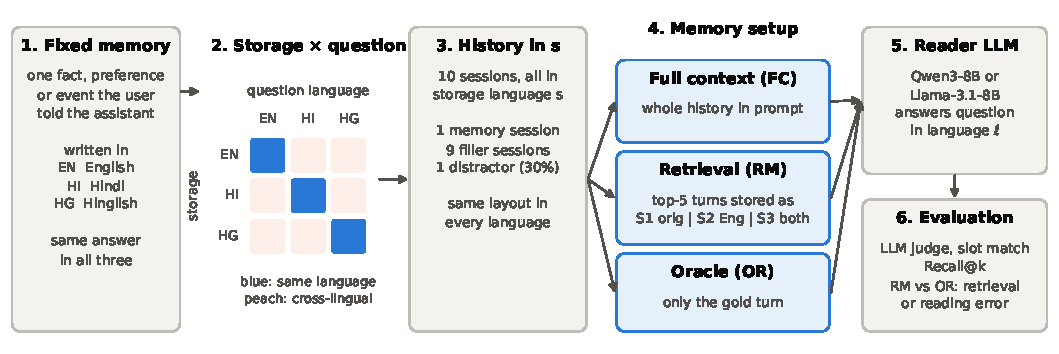
\includegraphics[width=\textwidth]{figures/fig0_method_overview.pdf}
\caption{Overview of the evaluation. A fixed memory is written in three languages, placed in a history in the storage language and queried in a question language. Comparing retrieval memory with the oracle separates retrieval errors from reading errors.}
\label{fig:method}
\end{figure*}

% ---------------------------------------------------------------------
\section{Related Work}
\label{sec:related}

\subsection{Long-term memory in LLM agents}
Long-term memory systems treat memory as an explicit store that the agent writes, retrieves and updates~\citep{packer2023memgpt,zhong2024memorybank}.
Benchmarks test question answering over long conversations~\citep{maharana2024locomo,wu2025longmemeval}. LongMemEval also decomposes memory into indexing, retrieval and reading stages~\citep{wu2025longmemeval}.
This body of work shows that agents lose information over long horizons, but it measures that loss in English only.

Our work keeps the memory task of these benchmarks and derives its items from LongMemEval.
We add a controlled language dimension that none of them varies.
We also reuse the retrieval and reading decomposition, and we measure it separately for each pair of storage and query languages.

\subsection{Cross-lingual retrieval and question answering}
Cross-lingual question answering pairs a question in one language with a context in another.
MLQA introduced this setting over parallel Wikipedia paragraphs in seven languages, including Hindi~\citep{lewis2020mlqa}.
These studies concern encyclopedic or news documents rather than memories that a user disclosed in conversation.
We study personal memories that a user disclosed in conversation, and we vary the question language as well as the storage language.
Our English-translation condition tests whether a shared representation helps inside a memory store.

\subsection{Code-switching and multilingual agents}
Code-switching benchmarks established Hindi--English mixing as a research topic~\citep{khanuja2020gluecos}.
None of these studies evaluates memory.
A bilingual English--Vietnamese memory dataset mixes languages across events, but each question exists in one language only~\citep{nguyendang2026lhmemory}.
Table~\ref{tab:related} positions our work against the closest studies.

\begin{table}[t]
\centering\small\setlength{\tabcolsep}{3pt}
\begin{tabular}{lccccccc}
\toprule
Work & Mem & St & Q & Mt & \HI & CM & Rep \\
\midrule
LongMemEval & \yes & \no & \no & \no & \no & \no & \partly \\
LoCoMo & \yes & \no & \no & \no & \no & \no & \partly \\
EN/VI memory set & \yes & \partly & \partly & \no & \no & \partly & \no \\
MLQA & \no & \yes & \yes & \yes & \yes & \no & \no \\
\textbf{Ours} & \yes & \yes & \yes & \yes & \yes & \yes & \yes \\
\bottomrule
\end{tabular}
\caption{Positioning against the closest work. Mem means personal or agent memory, St and Q mean the storage and query languages vary, Mt means the content is matched across languages, \HI\ means Hindi is included, CM means code-mixed text is included and Rep means memory representations are compared. The symbols \yes, \partly\ and \no\ mean yes, partly and no.}
\label{tab:related}
\end{table}

% ---------------------------------------------------------------------
\section{Methodology}
\label{sec:method}

\subsection{Task formulation}
An \emph{item} consists of a personal memory, a question about it and a gold answer.
The memory is a user turn that states a fact, a preference or an event.
The gold answer comes with accepted variants in all three scripts.
For a storage language $s$, we write the entire conversation history in $s$.
The question arrives in a new session in a query language $\ell$.
The nine pairs $(s,\ell)$ form a grid with three monolingual cells on its diagonal and six cross-lingual cells.
For a reader and memory setup $r$, we compute cell accuracy over $N$ items as
\[
\operatorname{Acc}_{s,\ell}^{(r)} = \frac{1}{N}\sum_{i=1}^{N} y_{i,s,\ell}^{(r)},
\]
where $y_{i,s,\ell}^{(r)}$ is one when the judged answer to item $i$ is correct and zero otherwise. The cross-lingual gap reported in Table~\ref{tab:gap} is
\[
\Delta^{(r)}=\frac{1}{3}\sum_{s}\operatorname{Acc}_{s,s}^{(r)}-\frac{1}{6}\sum_{s\ne\ell}\operatorname{Acc}_{s,\ell}^{(r)}.
\]
A positive $\Delta^{(r)}$ therefore indicates lower accuracy after a language switch.

\subsection{Dataset construction}
We derive items from LongMemEval, which is released under the MIT licence~\citep{wu2025longmemeval}.
Its 64 single-session questions about user facts become \emph{fact} items.
Its 30 preference questions have open-ended answers, so we rewrite them as short-answer questions.
We build \emph{event} items from 87 user turns that contain an explicit calendar date.
We keep an item only if one user turn answers it, the answer is short, the answer is personal and the text translates naturally into Hindi.
The resulting pool holds 150 items, with 50 facts, 50 preferences and 50 events.
This paper reports a pilot with 30 of these items, ten of each type, and three unanswerable control questions.

Each item contains a memory turn, an assistant reply that never repeats the answer, a short follow-up exchange and two equivalent wordings of the question.
In 30\% of items we add a \emph{distractor}, which is a similar statement about another person with a different value, such as ``my sister's commute is only 20 minutes''.
Hindi verbs mark the gender of the speaker, so we fix the user's gender for each item and balance it within each memory type.
Hindi text uses Devanagari with brand names in Latin letters, and Hinglish uses Roman letters with Hindi grammar.
An LLM drafted the translations.
Automatic checks confirm that the answer appears in the memory turn in every language and never appears in the replies or questions.
They also confirm that each distractor contains its own value and that verb gender matches the user.
The full study will add independent human checks of the translated items.

\subsection{Conversation histories}
Each history contains ten sessions, which are the memory session and nine filler sessions taken from LongMemEval.
Qwen3-8B translated the filler sessions into Hindi and Hinglish.
A plain prompt produced Devanagari in 48\% of the Hinglish filler turns, so we added worked examples, a fallback that romanises the Hindi translation and a quality check that stops the run.
We write the filler in the storage language, so a Hindi memory never stands out against English text.
A fixed random seed per item chooses the filler sessions, the position of the memory and the position of the distractor, and these choices are identical in all three languages.

\subsection{Memory setups and representations}
We compare three ways of giving the model access to its memory.
In the \emph{full context} setup (FC), the whole history is part of the prompt.
In the \emph{retrieval memory} setup (RM), we index every user turn and show the model the five turns most similar to the question, ranked by the BGE-M3 embedding model~\citep{chen2024bgem3}.
RM uses one of three representations.
S1 stores the original text, S2 stores an English translation of each memory and translates the question as well, and S3 stores both versions.
In the \emph{oracle} setup (OR), the model receives only the correct turn and the distractor, if the item has one.
The oracle removes retrieval, so the difference between RM and OR measures retrieval errors, and the errors that remain under OR are reading errors.

% ---------------------------------------------------------------------
\section{Experimental Setup}
\label{sec:setup}

\subsection{Input and output}
Table~\ref{tab:io} shows one instance from the pilot.
The input consists of a fixed English instruction, the history or the retrieved memories, and the question.
The expected output is one short sentence that contains the gold answer, in any language or script.
Appendix~\ref{app:prompts} lists all prompts.

\begin{table*}[t]
\centering\small
\begin{tabularx}{\textwidth}{@{}>{\raggedright\arraybackslash}p{0.22\textwidth}X@{}}
\toprule
\textbf{Memory (Hindi, Devanagari)} & \hi{मैं आजकल रोज़ ऑफिस आते-जाते ऑडियोबुक्स सुनती हूँ, एक तरफ़ का सफ़र 45 मिनट का होता है।} \emph{Maiṃ ājakal roz office āte-jāte audiobooks suntī hūṃ, ek taraf kā safar 45 minat kā hotā hai.} (I listen to audiobooks while commuting. One side takes 45 minutes.) \\
\textbf{Distractor (Hindi, Devanagari)} & \hi{मेरी बहन का ऑफिस तो बस एक तरफ़ 20 मिनट दूर है।} \emph{Merī bahan kā office to bas ek taraf 20 minat dūr hai.} (My sister's office is only 20 minutes away each way.) \\
\textbf{Question (Hinglish, Roman)} & \emph{Mera office jaane mein ek side kitna time lagta hai?} (How long does my commute take each way?) \\
\textbf{Gold answer} & 45 minutes each way. The distractor value is 20 minutes. \\
\textbf{Llama output (Hindi)} & \hi{मुझे आपकी पिछली बातचीत की याद है, जहां आपने बताया था कि आपकी बहन का ऑफिस तो बस एक तरफ़ 20 मिनट दूर है।} \emph{Mujhe āpkī pichhlī bātcīt kī yād hai, jahāṃ āpne batāyā thā ki āpkī bahan kā office ek taraf 20 minat dūr hai.} (I recall that your sister's office is 20 minutes away.) Incorrect because it returns the distractor value. \\
\textbf{Qwen output (Hindi)} & \hi{एक तरफ़ का सफ़र 45 मिनट का होता है।} \emph{Ek taraf kā safar 45 minat kā hotā hai.} (One side takes 45 minutes.) Correct. \\
\bottomrule
\end{tabularx}
\caption{A complete pilot instance for the commute item. The memory and distractor are stored in Hindi, the question is asked in Hinglish and the reader receives the full history.}
\label{tab:io}
\end{table*}

\subsection{Models and inference}
The readers are Qwen3-8B~\citep{yang2025qwen3} with its reasoning mode disabled and Llama-3.1-8B-Instruct~\citep{grattafiori2024llama3}.
Both models officially support Hindi.
We use greedy decoding at 16-bit precision with vLLM~\citep{kwon2023vllm} on two NVIDIA T4 GPUs from the free Kaggle tier.
The pilot produces 4,158 answers per reader, which are 33 items in 9 cells with 7 setups and 2 wordings, and the full run takes about 1.5 hours.

\subsection{Baselines}
The monolingual diagonal is the reference for each cross-lingual cell.
Storage of the original text (S1) is the baseline for the English and dual representations.
BM25~\citep{robertson2009bm25}, a keyword-matching retriever, serves as a lexical baseline next to the embedding retrievers BGE-M3 and multilingual-E5~\citep{wang2024me5}.
The full-context setup is the baseline without a memory module, and the oracle is an upper bound for reading.

\subsection{Metrics and evaluation}
\emph{Accuracy} is the share of answers that an LLM judge labels correct.
\emph{Recall@k} is the share of questions for which the correct memory turn appears among the top $k$ retrieved turns.
\emph{Reading error} is the share of wrong answers among questions where retrieval succeeded.
We also count \emph{distractor errors}, \emph{false abstentions}, which are ``I don't know'' answers to answerable questions, and \emph{invented answers} to the unanswerable controls.
The \emph{noise floor} is the rate at which the two equivalent wordings of a question receive different scores.
We pair all comparisons by item, report 95\% bootstrap confidence intervals and use exact sign tests~\citep{mcnemar1947} with Holm correction for multiple tests~\citep{holm1979}.

Automated evaluation covers answer matching against the accepted variants, retrieval ranks and the detection of the answer's script.
An LLM judge~\citep{zheng2023judging}, Qwen3-14B, labels every answer as correct, incorrect or no answer.
We sampled 200 answers for judge validation, but the independent human labels have not yet been collected.
Thus, the pilot accuracy values are judge-labelled estimates.
The main study will use two human annotators to validate the judge before reporting final results.
Our ablations vary the memory setup, the representation, the retriever and the wording of the question.

% ---------------------------------------------------------------------
\section{Results}
\label{sec:results}

\begin{figure*}[t]
\centering
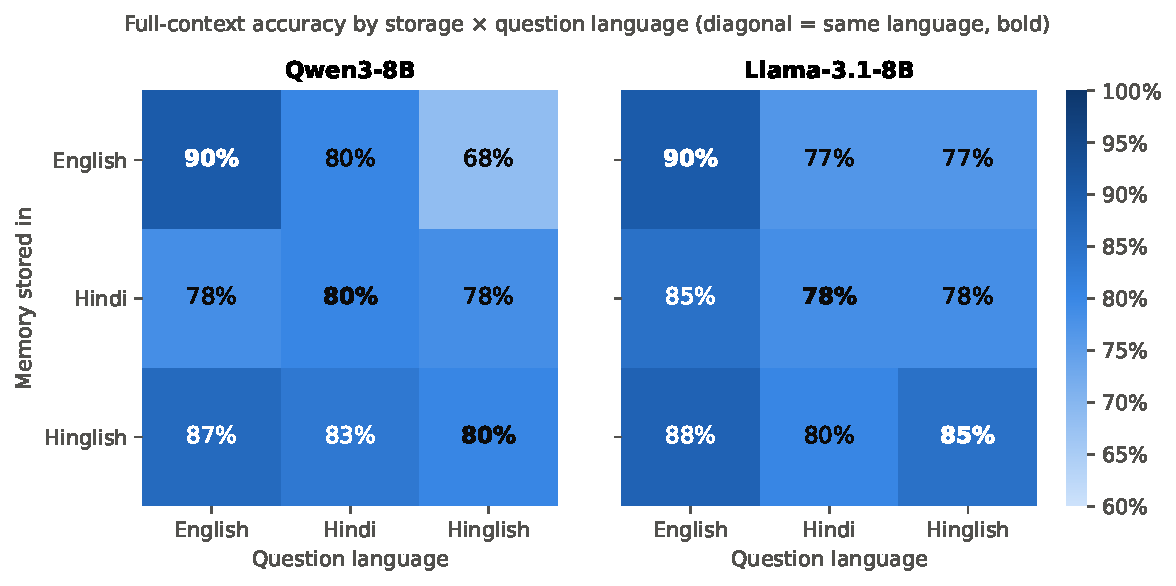
\includegraphics[width=0.82\textwidth]{figures/fig1_fc_accuracy_heatmap.pdf}
\caption{Full-context accuracy for each pair of storage and question language. Each cell covers 30 items with two wordings each. Bold cells are monolingual.}
\label{fig:heatmap}
\end{figure*}

\subsection{Cross-lingual accuracy}
Table~\ref{tab:gap} compares monolingual and cross-lingual accuracy for each setup, and Figure~\ref{fig:heatmap} shows the full-context grid.
In full context, cross-lingual accuracy is about four points lower for both models, but both confidence intervals include zero.
The two equivalent wordings of a question disagree on 18\% to 24\% of items in this setup, so a four-point difference lies within the noise of a 30-item pilot.

The retrieval and oracle setups are close to their ceiling.
BGE-M3 places the correct memory among the top five turns in 97\% to 100\% of questions in every cell, so retrieval rarely fails.
This ceiling motivates a harder retrieval setting in the main study.
The weakest single cell in Figure~\ref{fig:heatmap} is Qwen with English storage and a Hinglish question, at 68\%.

\begin{table}[t]
\centering\small\setlength{\tabcolsep}{4pt}
\begin{tabular}{llccc}
\toprule
Reader & Setup & Mono & Cross & Gap [95\% CI] \\
\midrule
\multirow{7}{*}{Qwen3} & FC & 83.3 & 79.2 & 4.2 [$-$0.6, 9.2] \\
 & RM-S1 & 91.1 & 89.4 & 1.7 [$-$0.8, 4.4] \\
 & RM-S2 & 92.2 & 88.3 & 3.9 [0.6, 7.8] \\
 & OR-S1 & 95.0 & 95.6 & $-$0.6 [$-$3.6, 2.5] \\
 & RM-S3 & 92.2 & 91.4 & 0.8 [$-$1.9, 3.6] \\
 & OR-S2 & 97.2 & 95.6 & 1.7 [0.3, 3.3] \\
 & OR-S3 & 97.8 & 96.9 & 0.8 [$-$1.4, 3.1] \\
\midrule
\multirow{7}{*}{Llama} & FC & 84.4 & 80.8 & 3.6 [$-$1.1, 8.6] \\
 & RM-S1 & 94.4 & 94.7 & $-$0.3 [$-$3.9, 3.3] \\
 & RM-S2 & 96.7 & 96.7 & 0.0 [$-$2.2, 2.2] \\
 & OR-S1 & 97.8 & 96.9 & 0.8 [$-$1.7, 3.3] \\
 & RM-S3 & 96.7 & 95.6 & 1.1 [$-$2.5, 4.4] \\
 & OR-S2 & 97.8 & 98.3 & $-$0.6 [$-$2.2, 0.8] \\
 & OR-S3 & 97.2 & 97.2 & 0.0 [$-$2.8, 2.5] \\
\bottomrule
\end{tabular}
\caption{Accuracy in percent on monolingual and cross-lingual cells, paired by item, for every reader and memory setup.}
\label{tab:gap}
\end{table}

\subsection{Language direction}
We compare each cross-lingual cell in Figure~\ref{fig:heatmap} with its mirror image.
A memory stored in Hinglish and asked about in English is answered correctly more often than the reverse, on 11 items against 2 items, with a difference of 18 points and a 95\% interval from 7 to 32 points.
The exact test gives $p=0.022$, but we ran 42 such tests, and the effect is not significant after Holm correction.

Llama points in the same direction, on 8 items against 3.
We treat this pattern as a hypothesis for the main study.

\subsection{Question language and code-switching}
Table~\ref{tab:qvs} splits full-context accuracy by one language at a time.
English questions score highest for both models, while Hindi and Hinglish questions score lower, with the lowest result for Hinglish questions to Qwen.
Code-switching therefore hurts mainly when it appears in the question.

Accuracy varies little across storage languages, and Hinglish storage scores slightly higher than English or Hindi storage for both models.

\begin{table}[t]
\centering\small\setlength{\tabcolsep}{5pt}
\begin{tabular}{lcccccc}
\toprule
 & \multicolumn{3}{c}{By question language} & \multicolumn{3}{c}{By storage language} \\
\cmidrule(lr){2-4}\cmidrule(lr){5-7}
Reader & \EN & \HI & \HG & \EN & \HI & \HG \\
\midrule
Qwen3 & 85.0 & 81.1 & 75.6 & 79.4 & 78.9 & 83.3 \\
Llama & 87.8 & 78.3 & 80.0 & 81.1 & 80.6 & 84.4 \\
\bottomrule
\end{tabular}
\caption{Full-context accuracy in percent, averaged over the other language.}
\label{tab:qvs}
\end{table}

\begin{figure*}[t]
\centering
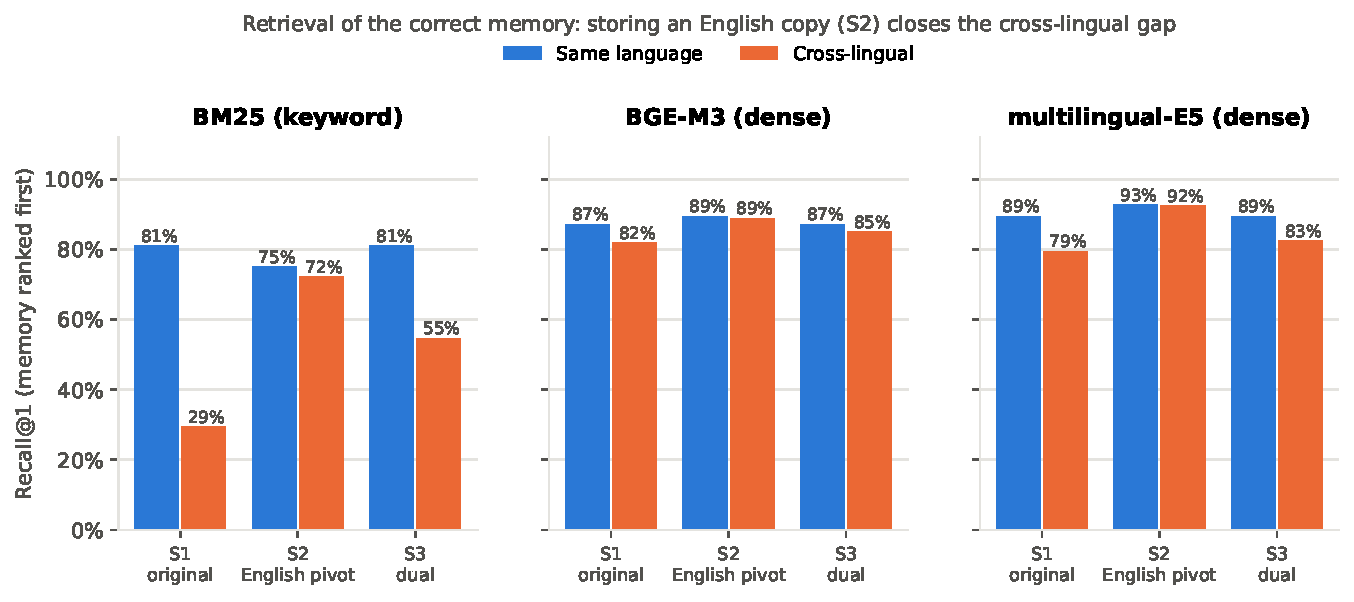
\includegraphics[width=0.9\textwidth]{figures/fig2_retrieval_recall_at_1.pdf}
\caption{Recall@1 of the correct memory for each retriever and representation, on monolingual and cross-lingual cells.}
\label{fig:retrieval}
\end{figure*}

\subsection{Memory representation}
Figure~\ref{fig:retrieval} shows how often each retriever ranks the correct memory first.
With the original text, BM25 ranks the correct memory first in 81\% of monolingual questions but in only 29\% of cross-lingual ones, because English and Devanagari share no words.
Storing an English copy raises the cross-lingual rate to 72\%, and storing both versions reaches 55\%.

They find the memory among the top five in almost every case, but they still rank it first less often across languages, with BGE-M3 falling from 87\% to 82\% and multilingual-E5 from 89\% to 79\%.
The English copy removes this loss for both retrievers.
Retrieval is rarely the bottleneck in the pilot, since Qwen misses the memory in 0.8\% of cross-lingual S1 questions but answers 9.8\% of the retrieved cases wrongly.

\subsection{Error analysis}
Most full-context errors are false abstentions.
Of 105 errors by Qwen and 97 errors by Llama, 69 and 71 respectively are ``I don't know'' answers, so the models fail to find the memory more often than they misremember it.
Distractor errors are rare, and Table~\ref{tab:io} shows one in which Llama reports the sister's commute instead of the user's.
Events with explicit dates are the easiest memory type, and preferences are the hardest.

On the unanswerable controls, Qwen gives a specific answer in 18.5\% of cases and Llama in 7.9\%.
Qwen answers English questions in English in 96\% of cases, while Llama answers them in Hindi or Hinglish in 45\% of cases.
Both models answer a quarter or more of Hinglish questions in Devanagari script.

Storage in Hindi is also more expensive.
The same history needs 4.1 times as many tokens in Hindi as in English for the Qwen tokenizer and 2.3 times as many for the Llama tokenizer, as Figure~\ref{fig:tokens} shows.
A Hindi history is therefore longer for the model, which the main study must report as a property of the language.

\begin{figure}[t]
\centering
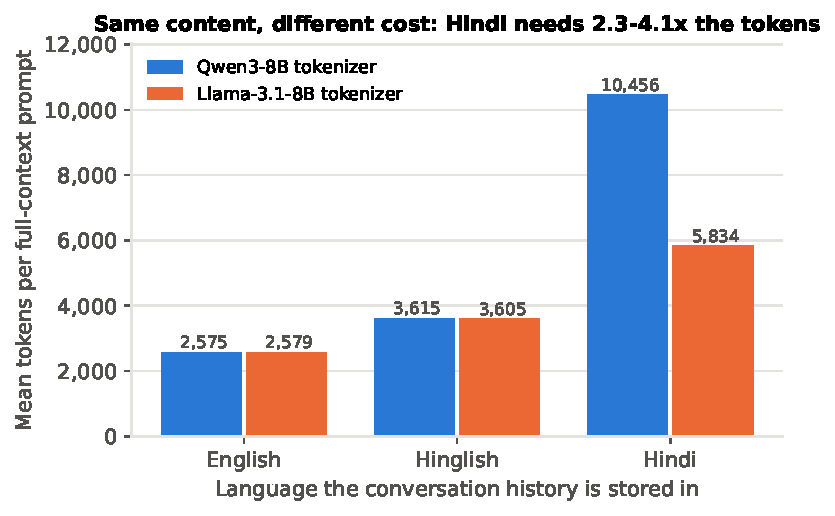
\includegraphics[width=0.9\columnwidth]{figures/fig3_token_cost.pdf}
\caption{Mean number of tokens per full-context prompt by storage language.}
\label{fig:tokens}
\end{figure}

\subsection{Summary of findings}
The pilot does not establish a reliable overall accuracy loss from changing language because the estimated four-point full-context gap is within the uncertainty of 30 items. It does show a clear retrieval representation effect. An English copy of a memory raises BM25 cross-lingual Recall@1 from 29\% to 72\%. Question language affects full-context accuracy more than storage language, and false abstentions account for most errors. Hindi histories also require substantially more tokens than equivalent English histories.

\subsection{Lessons and next steps}
\label{sec:next}
The pilot validated the pipeline and identified practical constraints in translation quality, token counting and Kaggle disk use.
The main study will use all 150 items, which gives 80\% power for paired gaps of about 12 points.
It will make retrieval harder with about 20 sessions per history and distractors in half of the items, because 30 Hindi sessions would exceed the context length of Qwen3-8B.
It will also add a human evaluation with two annotators and ablations on longer histories, indirect questions, Devanagari digits and English-framed Hinglish.

% ---------------------------------------------------------------------
\section{Conclusion}
We presented a controlled evaluation of cross-lingual agent memory that holds each personal memory fixed while varying its storage and query language across English, Hindi and Hinglish.
A 30-item pilot shows that an English representation of each memory protects retrieval across scripts.
It also shows that the language of the question matters more than the language of storage, and that most failures are false abstentions.
The overall cross-lingual gap is small compared with the measurement noise at pilot scale, and our 150-item study is designed to measure it.

% ---------------------------------------------------------------------
\section*{Limitations}
This study is a pilot, and its 30 items give limited statistical power.
An LLM drafted the Hindi and Hinglish items, and independent human checks have not yet been completed.
Machine translation produced the filler sessions, which contain minor errors, although the evaluation never scores them.
The pilot uses an LLM judge, and its human validation is still pending.
The judge also accepted two invented answers to unanswerable questions, so the reported rates of invented answers may be too low.
The source data from LongMemEval reflects mostly American contexts.
We tested two open models with eight billion parameters only, and retrieval was near its ceiling, so the pilot cannot yet show how retrieval errors propagate to answers.

\section*{Acknowledgements}
We thank Kaggle for free GPU access and the authors of LongMemEval for releasing their data.

\noindent\textbf{AI Use Statement.}
As the course permits, we used AI tools to assist with literature discovery, experimental design, dataset drafting, translation, code development, analysis and manuscript preparation.
The author is responsible for verifying the methods, calculations and claims before submission.

\bibliography{custom}

% ---------------------------------------------------------------------
\clearpage
\onecolumn
\appendix

\section*{Appendix}
\label{app:prompts}
This appendix lists the prompt templates used by the pilot pipeline. Braced fields are filled at runtime.

\subsection*{Reader Prompts}
\paragraph*{System prompt}
\begin{quote}\footnotesize\ttfamily
You are a personal assistant with memory of your past conversations with this user.\par
Answer the user's question using only what the user told you in past conversations.\par
Answer in one short sentence, in the same language as the question.\par
If the information is not in the past conversations, say that you don't know.
\end{quote}

\paragraph*{Full-context user message}
\begin{quote}\footnotesize\ttfamily
Past conversations:\par
[Session 1]\par
User: \{user turn\}\par
Assistant: \{assistant turn\}\par
\ldots\par
Current question: \{query\}
\end{quote}

\paragraph*{Retrieval and oracle user message}
\begin{quote}\footnotesize\ttfamily
Relevant memories from past conversations (may be incomplete or irrelevant):\par
1. \{memory 1\}\par
2. \{memory 2\}\par
\ldots\par
Current question: \{query\}
\end{quote}
For the dual representation, each retrieved memory is formatted as \texttt{\{original\} (English \{translation\})}.

\subsection*{Judge Prompts}
\paragraph*{Answerable-item judge}
\begin{quote}\footnotesize\ttfamily
You are grading an assistant's answer about a user's personal information.\par
Question: \{query\}\par
Gold answer: \{gold answer\}\quad Accepted forms: \{aliases\}\par
Assistant answer: \{response\}\par
The answer may be in English, Hindi (Devanagari) or Hinglish (romanized). Judge meaning, not language.\par
Reply with exactly one word:\par
CORRECT - states the gold information without contradiction\par
INCORRECT - wrong, incomplete, lists several candidates, or contradicts the gold\par
NO\_ANSWER - says it does not know / has no information
\end{quote}

\paragraph*{Unanswerable-item judge}
\begin{quote}\footnotesize\ttfamily
You are grading an assistant's answer about a user's personal information.\par
Question: \{query\}\par
Gold answer: the user never told the assistant this, so the assistant should say it does not know.\par
Assistant answer: \{response\}\par
The answer may be in English, Hindi (Devanagari) or Hinglish (romanized). Judge meaning, not language.\par
Reply with exactly one word:\par
ANSWERED - gives some specific answer to the question\par
NO\_ANSWER - says it does not know / has no information
\end{quote}

\subsection*{Translation Prompts}
\paragraph*{English pivot translation}
\begin{quote}\footnotesize\ttfamily
Translate the following text to English. It may be Hindi, Hinglish (romanized Hindi) or English.\par
Keep names, numbers and dates exactly. Output only the translation.\par
Text: \{text\}
\end{quote}

\paragraph*{Hindi filler translation}
\begin{quote}\footnotesize\ttfamily
Translate the following text into natural, conversational Hindi written in Devanagari script.\par
Keep brand and product names in Latin script, write person and place names in Devanagari, and keep digits as 0-9. Output only the translation.\par
Text: \{text\}
\end{quote}

\paragraph*{Hinglish filler rewrite}
\begin{quote}\footnotesize\ttfamily
Rewrite the following text in Hinglish: the casual Hindi-English mix used in Indian chat, with Hindi grammar, common English words mixed in, written ONLY in Roman (Latin) script. Never use Devanagari. Keep names, numbers and brand names unchanged. Output only the rewritten text.\par
Text: \{text\}
\end{quote}

\end{document}
